\documentclass[9pt,twocolumn]{extarticle}
\usepackage[margin=0.55in]{geometry}
\usepackage{amsmath,amssymb}
\usepackage{graphicx}
\usepackage{booktabs}
\usepackage{titlesec}
\usepackage{times}
\usepackage{enumitem}
\setlist{nosep,leftmargin=*}
\titlespacing{\section}{0pt}{4pt}{2pt}
\titlespacing{\subsection}{0pt}{3pt}{1pt}
\title{\vspace{-1.5em}\textbf{\large Adaptive Token-Aware KV Cache Compression with
Asymmetric Key/Value Quantization Granularity}\vspace{-0.5em}}
\author{\normalsize Chandan Munjal \\ \footnotesize chandanmunjal@gmail.com}
\date{}
\pagestyle{empty}

\begin{document}
\maketitle
\vspace{-2.2em}

\noindent\textbf{Abstract.} We present AdaptiveKVCache: a never-evict KV cache that
continuously reassigns each cached token to FP16/INT8/INT4 by a decayed importance
score (tokens can be promoted back up, unlike hard eviction), with keys quantized
per-channel (chunked) and values per-token within each tier. On Qwen2.5-1.5B-Instruct
and Phi-3-mini-4k-instruct: $\le$0.16\% perplexity degradation at
$\sim$40\% memory reduction; per-channel K quantization cuts K-MAE by up to
17.3\% vs.\ per-token K at matched compression (model-dependent -- see table).

\section{Method}
Every token $i$ gets score $s_i \leftarrow \gamma s_i + (1-\gamma) N m_i$ (Eq.~1), with
$m_i$ from attention mass, attention$\times\lVert v\rVert_1$ (VATP), or attention-free
key dissimilarity from the running mean key (KeyDiff, default). Every $R$ tokens,
non-recent/non-sink tokens are ranked by $s_i$ and split into FP16/INT8/INT4 fractions
$f_{16}, f_8, 1{-}f_{16}{-}f_8$ (Eq.~2). Quantization is asymmetric min--max,
$q = \mathrm{clip}(\mathrm{round}((x{-}z)/s), q_{\min}, q_{\max})$, with keys grouped
per-channel over chunks of $g_K$ tokens (exploiting per-channel K outliers) and values
grouped per-token (Fig.~1).

\begin{center}
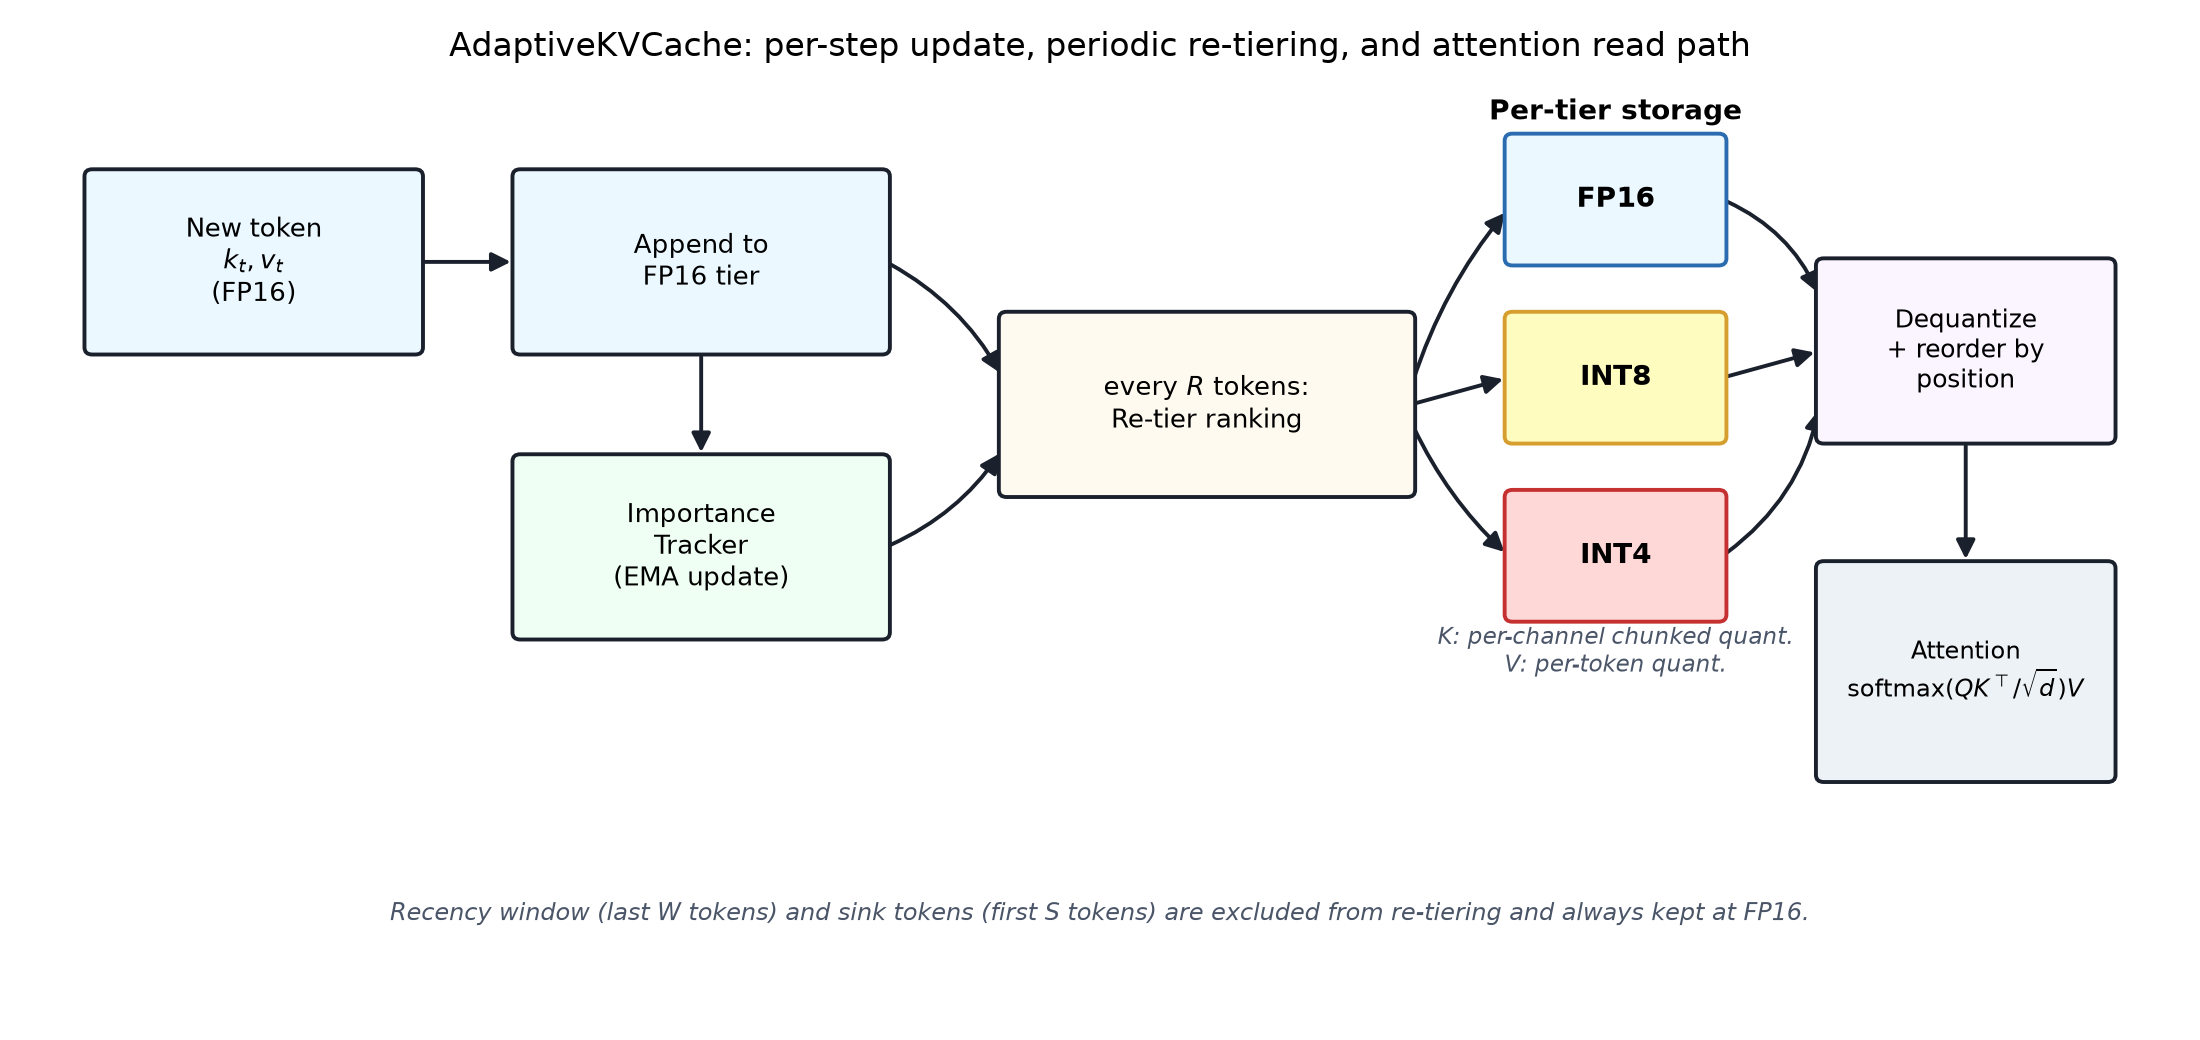
\includegraphics[width=0.48\textwidth]{figures/architecture.png}
\end{center}
\vspace{-0.3em}
{\footnotesize Fig.~1: per-step update $\rightarrow$ EMA importance $\rightarrow$
periodic re-tier $\rightarrow$ per-tier quantized storage $\rightarrow$ dequant/reorder
for attention.}

\section{Results}
Config: $W{=}32, S{=}4, f_{16}{=}f_8{=}0.30, R{=}16$, key\_diversity mode, greedy decoding,
FP16 \texttt{DynamicCache} baseline.

\begin{center}
\small
\begin{tabular}{lccc}
\toprule
Model & PPL degr.\ & Mem.\ reduction & K-MAE $\Delta$ (channel vs.\ token) \\
\midrule
Qwen2.5-1.5B & 0.16\% & 39.6\% & +17.3\% \\
Phi-3-mini & 0.02\% & 39.4\% & +0.2\% \\
\bottomrule
\end{tabular}
\end{center}

NIAH (distractor-hardened, 3 decoys/cell) and LongBench narrativeqa F1
(context-truncation fixed to preserve the question) show baseline and adaptive tracking
each other exactly, model for model: NIAH mean accuracy 0.62/0.62 (Qwen) and 0.02/0.02
(Phi-3); LongBench F1 0.080/0.094 (Qwen) and 0.078/0.077 (Phi-3) (baseline/adaptive). No
relative degradation on either task -- though Phi-3's 0.02 NIAH accuracy is a floor
effect (task too hard for this model at this difficulty), not evidence of strong absolute
retrieval; see full report.

\section{Takeaway}
Continuous bidirectional tiering (vs.\ hard eviction) plus K/V-asymmetric quantization
granularity keeps LM-quality degradation (perplexity) comfortably under 1\% at
$\sim$40\% memory reduction; downstream task metrics (NIAH, LongBench) required fixing
two independent evaluation-harness bugs (a ceiling effect and a question-truncation
bug) before they could be trusted as evidence either way.

\end{document}
